\documentclass[reprint,english,notitlepage]{revtex4-1}  % defines the basic parameters of the document

% if you want a single-column, remove reprint

% allows special characters (including æøå)
\usepackage[utf8]{inputenc}
\usepackage[english]{babel}

%% note that you may need to download some of these packages manually, it depends on your setup.
%% I recommend downloading TeXMaker, because it includes a large library of the most common packages.

\usepackage{physics,amssymb}  % mathematical symbols (physics imports amsmath)
\usepackage{graphicx}         % include graphics such as plots
\usepackage{xcolor}           % set colors
\usepackage{hyperref}         % automagic cross-referencing (this is GODLIKE)
\usepackage{tikz}             % draw figures manually
\usepackage{listings}         % display code
\usepackage{subfigure}        % imports a lot of cool and useful figure commands
\usepackage{cprotect}
\usepackage{float}


% defines the color of hyperref objects
% Blending two colors:  blue!80!black  =  80% blue and 20% black
\hypersetup{ % this is just my personal choice, feel free to change things
    colorlinks,
    linkcolor={red!50!black},
    citecolor={blue!50!black},
    urlcolor={blue!80!black}}

%% Defines the style of the programming listing
%% This is actually my personal template, go ahead and change stuff if you want
\lstnewenvironment{python}{
	\lstset{ %
		inputpath=,
		backgroundcolor=\color{white!88!black},
		basicstyle={\ttfamily\scriptsize},
		commentstyle=\color{magenta},
		language=Python,
		morekeywords={True,False},
		tabsize=4,
		stringstyle=\color{green!55!black},
		frame=single,
		keywordstyle=\color{blue},
		showstringspaces=false,
		columns=fullflexible,
		keepspaces=true}
}{}

\lstnewenvironment{cpp}{
	\lstset{ %
		inputpath=,
		backgroundcolor=\color{white!88!black},
		basicstyle={\ttfamily\scriptsize},
		commentstyle=\color{magenta},
		language=C++,
		morekeywords={True,False},
		tabsize=4,
		stringstyle=\color{green!55!black},
		frame=single,
		keywordstyle=\color{blue},
		showstringspaces=false,
		columns=fullflexible,
		keepspaces=true}
}{}

\lstset{literate=
  {á}{{\'a}}1 {é}{{\'e}}1 {í}{{\'i}}1 {ó}{{\'o}}1 {ú}{{\'u}}1
  {Á}{{\'A}}1 {É}{{\'E}}1 {Í}{{\'I}}1 {Ó}{{\'O}}1 {Ú}{{\'U}}1
  {à}{{\`a}}1 {è}{{\`e}}1 {ì}{{\`i}}1 {ò}{{\`o}}1 {ù}{{\`u}}1
  {À}{{\`A}}1 {È}{{\'E}}1 {Ì}{{\`I}}1 {Ò}{{\`O}}1 {Ù}{{\`U}}1
  {ä}{{\"a}}1 {ë}{{\"e}}1 {ï}{{\"i}}1 {ö}{{\"o}}1 {ü}{{\"u}}1
  {Ä}{{\"A}}1 {Ë}{{\"E}}1 {Ï}{{\"I}}1 {Ö}{{\"O}}1 {Ü}{{\"U}}1
  {â}{{\^a}}1 {ê}{{\^e}}1 {î}{{\^i}}1 {ô}{{\^o}}1 {û}{{\^u}}1
  {Â}{{\^A}}1 {Ê}{{\^E}}1 {Î}{{\^I}}1 {Ô}{{\^O}}1 {Û}{{\^U}}1
  {œ}{{\oe}}1 {Œ}{{\OE}}1 {æ}{{\ae}}1 {Æ}{{\AE}}1 {ß}{{\ss}}1
  {ű}{{\H{u}}}1 {Ű}{{\H{U}}}1 {ő}{{\H{o}}}1 {Ő}{{\H{O}}}1
  {ç}{{\c c}}1 {Ç}{{\c C}}1 {ø}{{\o}}1 {å}{{\r a}}1 {Å}{{\r A}}1
  {€}{{\euro}}1 {£}{{\pounds}}1 {«}{{\guillemotleft}}1
  {»}{{\guillemotright}}1 {ñ}{{\~n}}1 {Ñ}{{\~N}}1 {¿}{{?`}}1
}



\usepackage{thmtools}
\DeclareMathOperator{\nullspace}{Nul}
\DeclareMathOperator{\collspace}{Col}
\DeclareMathOperator{\rref}{Rref}
%%\DeclareMathOperator{\dim}{Dim}

 % "meq": must be equal
\newcommand{\meq}{\overset{!}{=}}
\newcommand\numberthis{\addtocounter{equation}{1}\tag{\theequation}}

\newcommand{\R}{\mathbb{R}}
\newcommand*\Heq{\ensuremath{\overset{\kern2pt L'H}{=}}}
\usepackage{bm}
\newcommand{\uveci}{{\bm{\hat{\textnormal{\bfseries\i}}}}}
\newcommand{\uvecj}{{\bm{\hat{\textnormal{\bfseries\j}}}}}
\DeclareRobustCommand{\uvec}[1]{{%
  \ifcsname uvec#1\endcsname
     \csname uvec#1\endcsname
   \else
    \bm{\hat{\mathbf{#1}}}%
   \fi
}}
\usepackage[binary-units=true]{siunitx}

\makeatletter
\newcommand*{\balancecolsandclearpage}{%
  \close@column@grid
  \cleardoublepage
  \twocolumngrid
}
\makeatother

\newcounter{subproject}
\renewcommand{\thesubproject}{\alph{subproject}}
\newenvironment{subproj}{
\begin{description}
	\item[\refstepcounter{subproject}(\thesubproject)]
}{\end{description}}


\begin{document}
\title{Title}   % self-explanatory
\author{Eivind Støland, Anders P. Åsbø}               % self-explanatory
\date{\today}                             % self-explanatory
\noaffiliation                            % ignore this

\begin{abstract}
Abstract
\end{abstract}

\maketitle                                % creates the title, author, date


\tableofcontents

\section{Introduction} \label{sec:I}


\newpage

\section{Formalism} \label{sec:II}

\subsection{The Ising Model} \label{sec:II:a}

The Ising model is a mathematical model of ferromagnetic systems. It is based on a set of particles in a lattice with either spin up or down, and the energy that a particle has is dependent on other adjacent particles and on an external magnetic field if there is one. We will be working with this model in the canonical ensemble. The energy of a configuration of such a system is:

\begin{align*}
E &= -J \sum\limits_{<kl>}^N s_k s_l - B \sum\limits_k^N s_k \numberthis \label{eq:ising_general_total_energy} \, ,
\end{align*}

where $J$ is a parameter determining the strength of the interaction between adjacent particles, $B$ is a parameter determining the strength of the external magnetic field, and $N$ is the number of particles. The notation $<kl>$ in the first sum indicates that we should sum over all adjacent particles, and the values summed over, $s$, are the spins of particles, where the subscripts denote which particle it belongs to. The spins can be $s = \pm 1$, which we often denote with an arrow pointing upwards ($\uparrow$) for $s = +1$ and a downwards pointing arrow ($\downarrow$) for $s = -1$.

In order to further proceed we need a probability that governs the system. For this purpose, the Boltzmann distribution is used:

\begin{align*}
P_i (\beta) &= \frac{e^{-\beta E_i}}{Z} \numberthis \label{eq:boltzmann_dist} \, ,
\end{align*}

where $\beta = (k_B T)^{-1}$, $E_i$ the energy of a specific configuration of the system, $Z$ is the partition function, and the subscript $i$ denotes the configuration of the system. The parameter $\beta$ contains $k_B$ which is the Boltzmann constant, and $T$ is the temperature. The partition function is a normalization factor for the probability distribution, and is the sum of all the possible Boltzmann factors:

\begin{align*}
Z &= \sum\limits_i^M e^{-\beta E_i} \numberthis \label{eq:ising_partition_function} \, ,
\end{align*}  

where $M$ is the amount of microstates of the system. The magnetization of a given configuration is given by the sum of all the spins:

\begin{align*}
\mathcal{M}_i &= \sum\limits_j^N s_j \numberthis \label{eq:ising_magnetization}
\end{align*}

The mean of a general variable, $Q_i$, can be defined as:

\begin{align*}
\langle Q \rangle &= \sum\limits_i^M Q_i P_i(\beta) \numberthis \label{eq:mean}
\end{align*}

The variance of said variable can be defined as:

\begin{align*}
\text{Var}(Q) &= \langle Q^2 \rangle - \langle Q \rangle^2 \, , \numberthis \label{eq:variance} 
\end{align*}

which relates to the standard deviation $\sigma_Q$:

\begin{align*}
\sigma_q &= \sqrt{\text{Var}(Q)} \numberthis \label{eq:standard_deviation}
\end{align*}

The heat capacity at constant volume $C_V$ is related to the variance of the energy as follows:

\begin{align*}
C_V &= \frac{1}{k_B T^2} \text{Var}(E) = \frac{1}{k_B T^2} (\langle E^2 \rangle - \langle E \rangle^2) \, ,\numberthis \label{eq:heat_capacity}
\end{align*}

and the magnetic susceptibility $\chi$ is related to the variance of the magnetization:

\begin{align*}
\chi &= \frac{1}{k_B T} \text{Var}(\mathcal{M}) = \frac{1}{k_B T} ( \langle \mathcal{M}^2 \rangle - \langle \mathcal{M} \rangle^2) \numberthis \label{eq:magnetic_susceptibility}
\end{align*}

In the following section we look at a sample system.


\subsubsection{Periodic \( 2 \times 2 \) square lattice with no external field}

We look at a system where we have particles in a 2x2 square lattice. A configuration of the system can be visualized as follows: \newline

\begin{center}
\begin{tabular}{cc}
$\bullet$ & $\bullet$ \\
$\bullet$ & $\bullet$
\end{tabular}  , \newline
\end{center}

where we change the dots out for arrows to mark the spin of the particles. A sample configuration of the system can be visualized as follows: \newline

\begin{center}
\begin{tabular}{cc}
$\uparrow$ & $\downarrow$ \\
$\downarrow$ & $\uparrow$
\end{tabular}  . \newline
\end{center}


We can denote the spins of the system as $s_{ij}$, where the index $i$ corresponds to the row the particle is in and $j$ to the column. With periodic boundary conditions, the total energy of the system is then given by:

\begin{align*}
E &= -J ( 2s_{11}s_{12} + 2s_{11}s_{21} + 2s_{22}s_{21} + 2s_{22}s_{12}) \numberthis \label{eq:2x2_sq_lattice_en}
\end{align*}

As there are two possible states that the particles can be in, and there are four particles total, there are $2^4 = 16$ microstates. We are interested in the possible energies of this system, and they are listed in table \ref{table:2x2_sq_lattice_en_and_mag} along with the total magnetization, where we have used \eqref{eq:2x2_sq_lattice_en} and \eqref{eq:ising_magnetization} to calculate these values. Note that the values in this table are sorted by macrostate, as some of the microstates are effectively equal because of the symmetries of the system. There are a total of 6 configurations with two spins pointing upwards, but these do not all have the same energy, which means that the macrostate of the system cannot be uniquely determined by the amount of spins that point up (or down for that matter). If the two spins pointing upwards are adjacent the total energy is 0, and there are four such configurations. If the two spins are not adjacent the total energy is $8J$, and there are two such states. As there are then two macrostates (different energies) corresponding to two spins pointing up, we need a second identifier. The degeneracy of these macrostates differ, and so by listing both the degeneracy and the amount of spins pointing up we can uniquely determine all the macrostates of the system. This was used in the table.

\begin{table}[H]
\centering
\caption{This table contains the energies and total magnetization for all possible macrostates of the Ising model with a 2x2 square lattice of particles. The uniqueness of the macro state is determined by the amount of spins that are up (first column) and the degeneracy of said state (second column). Both are needed, as in the case with two spins pointing up there are four configurations with the two upwards pointing spins being adjacent, and two with them not being adjacent.} \label{table:2x2_sq_lattice_en_and_mag}
\begin{tabular}{|c|c|c|c|}
\hline
Spins up & Degeneracy & Energy & Magnetization \\
\hline
4 & 1 & -8J & 4 \\
3 & 4 & 0 & 2 \\
2 & 4 & 0 & 0 \\
2 & 2 & 8J & 0 \\
1 & 4 & 0 & -2 \\
0 & 1 & -8J & -4 \\
\hline
\end{tabular}
\end{table}


We can calculate the partition function of the system using \eqref{eq:ising_partition_function}:

\begin{align*}
Z &= \sum\limits_i^M e^{-\beta E_i} \\
&= 2 \bigg(e^{8J\beta} + e^{-8J\beta} \bigg) + 12 \\
&= 4\cosh(8J\beta) + 12
\end{align*}

The probability distribution of the system is thus:

\begin{align*}
P_i(\beta) &= \frac{e^{-\beta E_i}}{4\cosh (8J\beta) + 12}
\end{align*}

The expectation value for the energy can be found as follows:

\begin{align*}
\langle E \rangle &= \sum\limits_i^M E_i P_i(\beta) \\
 &= -8J \frac{2e^{8J\beta}}{4\cosh (8J\beta) + 12} + 8J \frac{2e^{-8J}}{4\cosh (8J\beta) + 12} \\
 &= -8J\frac{2(e^{8J\beta} - e^{-8J\beta})}{4\cosh (8J\beta) + 12} \\
 &= -8J\frac{\sinh(8J\beta) }{\cosh (8J\beta) + 3} \numberthis \label{eq:2x2_energy}
\end{align*}

It is simple to see that $\langle M \rangle = 0$, so a more interesting measure would be the expectation value of the absolute of the magnetization. The expectation value for the absolute value of the magnetization can be found similarly:

\begin{align*}
\langle |\mathcal{M}| \rangle &= \sum\limits_i^M |\mathcal{M}_i| P_i(\beta) \\
 &= \frac{2e^{8J\beta} + 4}{\cosh (8 J \beta) + 3} \numberthis \label{eq:2x2_abs_magnetization}
\end{align*}

In order to find the heat capacity it is first necessary to find the expectation value of squared energy:

\begin{align*}
\langle E^2 \rangle &= \sum\limits_i^M E_i^2 P_i(\beta) \\
&= 64J^2 \frac{\cosh(8J\beta)}{\cosh(8J\beta) + 3}
\end{align*}

This gives us the heat capacity by equation \eqref{eq:heat_capacity}:

\begin{align*}
C_V &= \frac{1}{k_B T^2} ( \langle E^2 \rangle - \langle E \rangle^2) \\
&= \frac{192J^2}{k_B T^2} \frac{\cosh(8J\beta)}{(\cosh(8J\beta) + 3)^2} \numberthis \label{eq:2x2_heat_capacity}
\end{align*}

Lastly we also want to find the magnetic susceptibility of the system. In order to do that we need to find:

\begin{align*}
\langle \mathcal{M}^2 \rangle &= \sum\limits_i \mathcal{M}_i^2 P_i(\beta) \\
&= 8 \frac{e^{8J\beta} + 1}{\cosh(8J\beta) + 3}
\end{align*}

This gives us the susceptibility by using equation \eqref{eq:magnetic_susceptibility}:

\begin{align*}
\chi &= \frac{1}{k_B T} ( \langle \mathcal{M}^2 \rangle - \langle \mathcal{M} \rangle^2 ) \\
&= \frac{8}{k_B T} \frac{e^{8J \beta} + 1}{\cosh( 8J \beta) + 3} \numberthis \label{eq:2x2_susceptibility}
\end{align*}

All of these values we have calculated here can be compared with numerical results later on in order to evaluate the veracity of the numerical results.


\subsubsection{Periodic square lattice with no external field in the thermodynamical limit} \label{sec:II:a:ii}

Solving the two-dimensional Ising model is a highly non-trivial task, and so we will only list the resulting expressions in the case where there is no external field. These expressions were found by Lars Onsager so we refer to his work \citep{L.Onsager1944} instead of performing the calculations ourselves. The partition function is given by the following:

\begin{align*}
Z_N &= [2\cosh(\beta J) e^I ]^N \, , \numberthis \label{eq:LO_partition_function}
\end{align*}

where: 

\begin{align*}
I &= \frac{1}{2\pi} \int_0^\pi d\phi \, \ln \bigg[\frac{1}{2}\bigg( 1 + ( 1 - \kappa^2 \sin^2 \phi)^{1/2} \bigg) \bigg] \, , 
\end{align*}

and:

\begin{align*}
\kappa &= \frac{2\sinh ( 2\beta J) }{\cosh^2(2\beta J)} \, ,
\end{align*}

and $N$ is the number of particles. This determines the mean energy:

\begin{align*}
\langle E \rangle &= -J \coth( 2\beta J) \bigg[ 1 + \frac{2}{\pi} (2\tanh^2 (2\beta J) - 1) K_1(\kappa) \bigg] \, , \numberthis \label{eq:LO_energy}
\end{align*}

where:

\begin{align*}
K_1 (\kappa) &= \int_0^{\pi/2} \frac{d\phi}{\sqrt{1 - \kappa^2 \sin^2 \phi}} \, .
\end{align*}

The heat capacity is derived from this quantity again, and is found to be:

\begin{align*}
C_V &= \frac{4k_B}{\pi} (\beta J \coth(2\beta J))^2 \bigg( K_1(\kappa) - K_2(\kappa) \\ 
& \quad - (1 - \tanh^2 (2\beta J) ) \bigg[ \frac{\pi}{2} + (2\tanh^2 (2\beta J) - 1)K_1(\kappa) \bigg] \bigg) \, , \numberthis \label{eq:LO_heat_capacity}
\end{align*}

where:

\begin{align*}
K_2(\kappa) &= \int_0^{\pi/2} d\phi \, \sqrt{1 - \kappa^2 \sin^2 \phi}
\end{align*}

The mean magnetization per spin is given by:

\begin{align*}
\langle \mathcal{M} / N \rangle &= \bigg[1 - \frac{(1- \tanh^2 (\beta J) )^4}{16\tanh^4 (\beta J)} \bigg]^{1/8} \, , \numberthis \label{eq:LO_magnetization_per_spin}
\end{align*}

when the temperature is lower than a specific critical value $T_C$. Above this value the mean magnetization per spin is zero.

These solutions have the interesting feature that they predict a phase transition at this critical temperature $T_C$. The heat capacity, magnetization and susceptibility all excibit a power law behaviour (\citep{Stanley1999}, \cite[chapter 2.1.2]{landau_binder_2014}) in the region where $T\to T_C$ and $T$ is close to $T_C$. Specifically the heat capacity behaves as:

\begin{align*}
C_V &\sim \bigg| T_C - T \bigg| ^{-\alpha} \, , \numberthis \label{eq:power_law_heat_capacity}
\end{align*} 

when $T\to T_C$ from below, and $T$ is close to $T_C$. It can be determined that the correct solution is $\alpha = 0$, meaning that this behaves according to the power law singularity in the thermodynamic limit. The magnetization per spin behaves as:

\begin{align*}
\langle \mathcal{M} / N \rangle &\sim (T_C - T)^{\beta} \, , \numberthis \label{eq:power_law_magnetization_per_spin}
\end{align*}

in the same region, and with $\beta \to 1/8$. Similarly the susceptibility can be shown to behave as:

\begin{align*}
\chi &\sim |T_C - T|^{-\gamma} \, , \numberthis \label{eq:power_law_susceptibility}
\end{align*}

in the same region, and with $\gamma \to 7/4$. The correlation function, $C(r)$, where the parameter $r$ defines the distance between spins, is a measure of how much the spins correlate with each other, and can be shown \citep{Stanley1999} to scale as:

\begin{align*}
C(r) &\sim  e^{-r/\xi} \, ,
\end{align*}

where $\xi$ is the correlation length. As we approach the critical temperature we expect this to decay slower, as a change in a spin should quickly correlate to a change in another spin elsewhere. As $r$ is only dependent on how far apart the spins are the only variable that can cause this to happen is the correlation length, meaning that it has to get large as we approach the critical temperature. Because of this it can be shown that close to the critical temperature the correlation length also exhibits power law behaviour  (this is shown in \citep{Stanley1999}, albeit by a different route than the one outlined here):

\begin{align*}
\xi (T) &\sim |T-T_C|^{-\nu} \, , \numberthis \label{eq:power_law_correlation_length_} 
\end{align*}

where $\nu$ is a constant. A phase transition such as the one that the Ising model predicts is characterized by a correlation length that spans the whole system, and thus this correlation length can also be connected to the size of the system if we are looking at a finite lattice:

\begin{align*}
\xi (T) &\propto L \, ,
\end{align*}

where $L$ is the amount of spins in one direction in this finite lattice. Connecting this with the previous result we can define a connection between the critical temperature in a finite lattice and the one in the thermodynamical limit:

\begin{align*}
T_C(L) - T_C(L= \infty) &\sim L^{-1/\nu} \, , \numberthis \label{eq:crit_temperature_finite_lattice} 
\end{align*}

where $\nu$ is the same constant as earlier. Combining this with the results for the heat capacity, the mean magnetization, and the magnetic susceptibility gives us the following relations in a finite lattice (\citep[p.78]{landau_binder_2014}):

\begin{align*}
C_V &\sim |T_C - T |^{-\alpha} \propto  L^{\alpha/\nu} \, , \numberthis \label{eq:finite_lattice_heat_capacity} \\
\langle \mathcal M \rangle &\sim (T-T_C)^\beta \propto L^{-\beta /\nu} \, , \numberthis \label{eq:finite_lattice_magnetization_per_spin} \\
\chi &\sim |T_C - T|^{-\gamma} \propto L^{\gamma/\nu} \, , \numberthis \label{eq:finite_lattice_susceptibility}
\end{align*}

where all variables are as defined earlier. We can use these relations to generate an estimate of $T_C(L)$, and if this is done for multiple $L$ we can estimate $T_C(L=\infty)$ by using equation \eqref{eq:crit_temperature_finite_lattice}. This allows us to calculate values for finite lattices numerically and relate them with results from the thermodynamic limit, which is essential as simulating an infinite is simply not possible. The analytical critical temperature with $\nu=1$ is (\citep{L.Onsager1944}):

\begin{align*}
\tilde{T}_C &= \frac{k_B T_C}{J} = \frac{2}{\ln(1 + \sqrt{2})} \approx 2.269 \, , \numberthis \label{eq:crit_temperature_analytical}
\end{align*}

where we have scaled the temperature $\tilde{T}_C$ using $k_B$ and $J$ so that it is a dimensionless quantity.


\subsection{The Ising model and the Metropolis algorithm} \label{sec:II:b}

One method of simulating a system in the Ising model is through a Markov Chain Monte Carlo setup, where we iterate and flip spins depending on the change in total energy that flipping said spins incur. The Metropolis algorithm \citep{Metropolis} is one such setup which we will explain in this section.

We propose a change in a set of spins will cause a change in the total configuration of the system. Changing the configuration of the system from one (denoted $a$) to another (denoted $b$) incurs a change in the total energy defined by $\Delta E = E_b - E_a$. If the change in energy is negative we instantly accept the new configuration, as the second law of thermodynamics states that the system should always move towards equillibrium (lowest energy) in a closed system. If however the change is positive (meaning that the system, we wish to let probabilities determine whether or not we accept the new configuration. We can calculate the probability of moving from configuration $a$ to $b$ by using the Boltzmann distribution \ref{eq:boltzmann_dist} ($P_i(T)$ where $i$ denotes the configuration of the system):

\begin{align*}
P_{a\to b}(T)  &= \frac{P_b (T) }{P_a (T)} = e^{-\beta \Delta E }\, . 
\end{align*}

In this case we assume that the change in energy is positive number, so this is always smaller than one as we wish for a probability. We then draw a random number $r$ between $0$ and $1$ using a random number generator, and compare this to the probability of the transition $P_{a\to b}(T)$. If $r\leq P_{a\to b} (T)$ we accept the new configuration, otherwise we keep the previous configuration. The process up to this point can be called a Monte Carlo cycle. The Monte Carlo cycle is performed a sufficient amount of times until the system has stabilized, which is characterized by the macroscopic variables of the system being stable.

As we can see we need to somehow calculate $P_{a\to b} (T)$ in every Monte Carlo cycle, and as this contains an exponential this is computationally expensive. We can, however, modify the Monte Carlo cycle in such a way that there only are set values of $\Delta E$, which means that we can precalculate $P_{a\to b} (T)$. Doing this will cause a massive speed up in the calculation. We have not yet outlined how we propose a new configuration, and this will also be covered by this same method.

If we flip only one spin at a time, there are only five possible changes in energy $\Delta E$. The difference in energy between the states of a two dimensional lattice when one spin is flipped can be calculated using \eqref{eq:ising_general_total_energy}. Assuming no outside magnetic field gives us the difference between states \(1\) and \(2\) as:

\begin{align*}
	\Delta E = E_{2} - E_{1} = \left(-J \sum\limits_{<kl>}^N s_k^{2} s_l^{2}\right) -
	\left(-J \sum\limits_{<kl>}^N s_k^{1} s_l^{1}\right),
\end{align*}

where a superscript is used to denote which state the respective spins belong to.

Since we are only interested in the difference in energy from flipping a single spin in the lattice, we can assume that \(s_{k}^{1} = s_{k}^{2} = s_{k}\). Thus we can rewrite \(\Delta E\) as
\begin{align*}
 	\Delta E = J \sum_{<kl>}^{N} s_{k} \left(s_{l}^{1} - s_{l}^{2}\right).
\end{align*}

Furthermore, any spin can only be \(\pm 1\) and spin \(s_{l}\) is flipped such that \(s_{l}^{2} = -s_{l}^{1}\). From this it follows that \begin{align*}
	\left(s_{l}^{1} - s_{l}^{2}\right) = \left(s_{l}^{1} + s_{l}^{1}\right) = 2s_{l}^{1}.
\end{align*}

The difference in energy can then be written as

\begin{align*}
 	\Delta E = 2Js_{l}^{1} \sum_{<k>}^{N} s_{k}, \numberthis \label{eq:delta_e}
\end{align*}

where we only sum over \(k\), since only one spin \(s_{l}\) is flipped.
For a two dimensional lattice, each spin only has four neighbours, thus we can write out the sum for any randomly chosen \(s_{l}\) with neighbours \(s_{a}, s_{b}, s_{c}, s_{d}\) as

\begin{align*}
	\Delta E = 2Js_{l}^{1}\left(s_{a} + s_{b} + s_{c} + s_{d}\right) \\
	\Delta E = 2J(\pm 1)\left[(\pm 1) + (\pm 1) + (\pm 1) + (\pm 1)\right]
\end{align*}

From this we see that if all spins \(s_{k}\) have the same sign we get
\begin{align*}
	\Delta E = \pm 2J(\pm 4) = \pm 8J.
\end{align*}
If three of the spins \(s_{k}\) have the same sign we get
\begin{align*}
	\Delta E = \pm 2J(\pm 2) = \pm 4J.
\end{align*}
If two of the spins \(s_{k}\) have the same sign we get
\begin{align*}
	\Delta E = \pm 2J(0) = 0.
\end{align*}
Thus we only have five possible diffrences in energy between states when we only flip one spin. We can also visualize the possible transitions as follows:

\begin{align*}
E = -4J \quad \begin{array}{ccc}
& \uparrow & \\
\uparrow & \uparrow & \uparrow \\
& \uparrow &
\end{array} \quad \to \quad E = 4J \quad \begin{array}{ccc}
& \uparrow & \\
\uparrow & \downarrow & \uparrow \\
& \uparrow &
\end{array} \, ,
\end{align*}

with $\Delta E = 8J$, 

\begin{align*}
E = -2J \quad \begin{array}{ccc}
& \uparrow & \\
\downarrow & \uparrow & \uparrow \\
& \uparrow &
\end{array} \quad \to \quad E = 2J \quad \begin{array}{ccc}
& \uparrow & \\
\downarrow & \downarrow & \uparrow \\
& \uparrow &
\end{array} \, ,
\end{align*}

with $\Delta E = 4J$,

\begin{align*}
E = 0 \quad \, \quad \begin{array}{ccc}
& \uparrow & \\
\downarrow & \uparrow & \uparrow \\
& \downarrow &
\end{array} \quad \to \quad E = 0 \,\,\,\, \quad \begin{array}{ccc}
& \uparrow & \\
\downarrow & \downarrow & \uparrow \\
& \downarrow &
\end{array} \, ,
\end{align*}

with $\Delta E = 0$, 

\begin{align*}
E = 2J \quad \begin{array}{ccc}
& \downarrow & \\
\downarrow & \uparrow & \uparrow \\
& \downarrow &
\end{array} \quad \to \quad E = -2J \quad \begin{array}{ccc}
& \downarrow & \\
\downarrow & \downarrow & \uparrow \\
& \downarrow &
\end{array} \, ,
\end{align*}

with $\Delta E = -4J$, and lastly:

\begin{align*}
E = 4J \quad \begin{array}{ccc}
& \downarrow & \\
\downarrow & \uparrow & \downarrow \\
& \downarrow &
\end{array} \quad \to \quad E = -4J \quad \begin{array}{ccc}
& \downarrow & \\
\downarrow & \downarrow & \downarrow \\
& \downarrow &
\end{array} \, ,
\end{align*}

with $\Delta E = -8J$. These are the only possible changes in energy. The other possible transitions are the ones above but in reverse, and the energy change is then just what is listed, but with the sign being flipped. 

With this in mind we can precalculate all the probabilities $P_{a \to b} (T)$ and use these. In the case where $\Delta E < 0$ we have that $P_{a\to b} (T) > 1$, which means that it seizes to be a proper probability, but if we draw a random number and compare it to this as outlined earlier, the test will always pass if $\Delta E < 0$, meaning that we do not have to handle this as a special case. In a two-dimensional system it is beneficiary to denote the spins as matrix elements $s_{ij}$ where $i$ is the lattice position of the spin in the $x$-direction and similarly for $j$ in the $y$-direction. With this notation we can establish an expression for the energy change from flipping spin $s_{ij}$:

\begin{align*}
\Delta E &= -2J s_{ij} \bigg( s_{i,j+1} + s_{i,j-1} + s_{i+1,j} + s_{i-1,j} \bigg) \numberthis \label{eq:singleflip_energy_change}
\end{align*}

A problem we encounter at this point is how we model the periodic boundary conditions. If we use a square lattice, we can use the amount of spins in a dimension $L$ and the modulo operator to define a function $f(i,k)$ that takes a valid index $i$ and what is to be added to it $k$, and returns the correct index on the other side of the lattice if it is out of bounds:

\begin{align*}
f(i) &= (i+k+L)\%L \, , \numberthis \label{eq:periodic}
\end{align*}

where \% is the modulo operator in this case. Note that we add $L$ to the total as well, as the function could return a negative value if $k$ was negative otherwise. The function might still return a negative value, but we have assumed here that $|k|$ is never larger than $L$. 
 
We have established that flipping one spin at a time is beneficial to the speed of the calculation. For larger systems this is a very small change, and so it is a good idea to flip more than one spin in each Monte Carlo cycle. Also if we want a more random process each cycle, we can also pick random spins that we attempt to flip, which we also choose to do later on. Exactly how all this is performed is outlined in section \hyperref[sec:III]{III}.

Every time a spin is flipped we need to update total energy and magnetization. The change in energy is $\Delta E$ and this can simply be added to the total. The difference in magnetization can be found using \eqref{eq:ising_magnetization}, and subtracting \(M_{2} - M_{1}\) (subscript one denotes the magnetization before the spin is flipped, and 2 the magnetization after): 

\begin{align*}
	\mathcal{M}_2 - \mathcal{M}_{1} &= \sum\limits_j^N s_j^{2} - \sum\limits_j^N s_j^{1} =
	\sum\limits_{j}^{N}\left(s_{j}^{2} - s_{j}^{1}\right).
\end{align*}

Because we assume only spin \(s_{l}\) is flipped when changing states, the difference in magnetization becomes:

\begin{align*}
 	\mathcal{M}_2 - \mathcal{M}_{1} = \left(s_{l}^{2} - s_{l}^{1}\right).
\end{align*} 

Using that \(s_{l}^{1} = - s_{l}^{2}\), we get:

\begin{align*}
	\mathcal{M}_2 - \mathcal{M}_{1} = \left(s_{l}^{2} + s_{l}^{2}\right) = 2s_{l}^{2},
\end{align*}

which gives that:

\begin{align*}
	\mathcal{M}_2 = \mathcal{M}_1 + 2s_{l}^{2} \numberthis \label{eq:delta_m}
\end{align*}


\newpage

\section{Method} \label{sec:III}

In this report we present simulations of the Ising model, in two dimensions with periodic boundary conditions and no external field, using the Metropolis algorithm. We have chosen to implement our solver as a class in C++ called \verb+IsingMetropolis+, with framework to operate said class using command line arguments in a main program in C++. Processing the results is done in Python, and all the simulations performed in this report is automated in Python as well. In this section we will discuss details on how key calculations are performed. In general we scale all equations used in these calculations such that $k_B = J = 1$. This makes it so that we do not need any natural constants at all, which simplifies the implementation significantly. The programs used are all linked to in appendix \hyperref[A]{A}.

\subsection{Details on calculations and key functions} \label{sec:III:a}

\subsubsection{Initialization of system} \label{sec:III:a:i}

Firstly, we will discuss how the system is initialized. We implemented two ways of initializing the spin matrix, total energy and magnetization. They are generated as follows:

\begin{cpp}
// Initiate spin matrix and magnetization
if (randspin) {
  for (int x = 0; x < n_spins; x++) {
    for (int y = 0; y < n_spins; y++) {
      spin_matrix(x,y) = (RNG(gen) >= 0.5) ? -1 : 1;
      M += spin_matrix(x,y);
    }
  }
} else {
  spin_matrix.ones();
  M = n_spins2;
}


// Initial energy
for(int y =0; y < n_spins; y++) {
  for (int x= 0; x < n_spins; x++){
    E -=  double(spin_matrix(y,x)*
          (spin_matrix(periodic(y,n_spins,-1),x) +
          spin_matrix(y,periodic(x,n_spins,-1))));
  }
}
\end{cpp}

Depending on the boolean variable \verb+randspin+ the spin-matrix is either generated as having all spins up (if \verb+randspin+ is false) or having a random spin configuration (if \verb+randspin+ is true). The spin matrix is an Armadillo \citep{Armadillo} integer matrix, which lets us use the \verb+ones()+ function to set all the spins to one. In this case the magnetization is simply the same as the total amount of spins which is stores in the variable \verb+n_spins2+. The random configuration is generated by using a double for loop, and random values drawn from the standard library function \verb+rand()+. In this case, every spin value is added to the variable that stores the magnetization (\verb+M+) in the same double for loop. The energy cannot be calculated at the same time as the spin matrix is being generated, as it needs all the neares neighbours to be generated already. Thus this calculation is separated into a secondary for loop, which is used in both cases. In general calculation of energy and magnetization is based on equations  \eqref{eq:ising_general_total_energy} and \eqref{eq:ising_magnetization} respectively.


\subsubsection{Performing a Monte Carlo sweep} \label{sec:III:a:ii}

The following code snippet performs one Monte Carlo sweep (flipping several spins, one at a time) based on the Metropolis algorithm on the system:

\begin{cpp}
std::random_device rd;
std::mt19937_64 gen(rd());
std::uniform_real_distribution<double> RNG(0.0, 1.0);
// Loop over all spins
for(int y =0; y < n_spins; y++) {
  for (int x= 0; x < n_spins; x++){

    // Get random indices
    int ix = int(RNG(gen)*(double)n_spins);
    int iy = int(RNG(gen)*(double)n_spins);

    // Calculate change in energy
    int deltaE =  2*spin_matrix(iy,ix)*
                  (spin_matrix(iy,periodic(ix,n_spins,-1))+
                  spin_matrix(periodic(iy,n_spins,-1),ix) +
                  spin_matrix(iy,periodic(ix,n_spins,1)) +
                  spin_matrix(periodic(iy,n_spins,1),ix));


    // Flip spin if new config is accepted
    if ( RNG(gen) <= w(deltaE+8) ) {
      spin_matrix(iy,ix) *= -1;


      // Update energy and magnetization if spin is flipped
      M += double(2*spin_matrix(iy,ix));
      E += double(deltaE);

      // Count accepted configs
      accepted_configs++;
    }
  }
}
\end{cpp}

The amount of spins that we attempt to flip, according to the condition from the Metropolis algorithm (see section \hyperref[sec:II:b]{II.B}), in one sweep is equal to the amount of spins in the system. The obvious solution in this case is to iterate through all the spins and attempt to flip each one, but a better solution is to let which spins we attempt to flip be random. In a physical context it is more realistic that all spins might flip at any point in time, meaning that any kind of ordering to which spin might flip would be unrealistic. To model this we use the Mersenne Twister random number generator \citep{MersenneTwister} which is implemented in the C++ standard library to draw random indices each iteration in the double for loop. 

At this point the change in energy is calculated. In order to apply the periodic boundary conditions an inline function \verb+periodic()+ is used. This function is equivalent to equation \eqref{eq:periodic}. Related to this equation the arguments it takes as input is $i$, $L$, and $k$, in that order. Adding to an existing valid index using this function returns the corresponding index on the other side of the lattice if it would otherwise be out of bounds on another side of the lattice.

Following this a random number is drawn, and if the probability of the energy transition is larger than this number then the spin is flipped. The Armadillo \citep{Armadillo} vector \verb+w+ stores the probabilities of the transitions and is calculated as follows:

\begin{cpp}
arma::vec w = arma::zeros(17);
for (int de = -8; de<= 8; de+=4) {
  w(de+8) = exp(-de/temperature(i));
}
\end{cpp} 

As the energy change is always an integer (we scaled the equations so that $J=1$) we can shift it by the lowest allowed value and use it as an index. This lets us access the probabilities using the energy change directly, removing the need for any calculation of any indices of \verb+w+ during the Monte Carlo sweep. Note that there are more values in \verb+w+ than there are allowed configurations. This is because the energy change can only be multiples of $2$. Dividing by two every time would cause unnecessary mathematical operations, so we instead define \verb+w+ to have twice as many elements as there are possible transitions between configurations.

If the random number drawn is less then the probability of the transition of configuration, the condition passes and the spin is flipped. If this is done the energy change is added to the total energy, and the magnetization is updated as well. A counter that keeps track of how many transitions that are accepted is also incremented. For further details on the algorithm used in this section, see section \hyperref[sec:II:b]{II.B}. 


\subsubsection{Running simulations} \label{sec:III:a:iii}

Simulations are performed by running the \verb+run()+ method of the \verb+IsingMetropolis+ class. As the program can run a simulation for a single temperature, or several simulations with different temperatures (all with the same lattice dimensions), this method is simply a wrapper that calls the correct function to run the simulation(s). In the case where a simulation is run for a single temperature, the following code snippet is used to run the simulation:

\begin{cpp}
double E = 0;
double M = 0;
arma::Mat<int> spin_matrix(n_spins,n_spins,arma::fill::ones);
arma::vec w = arma::zeros(17);
for (int de = -8; de<= 8; de+=4) {
  w(de+8) = exp(-de/temp);
}

initialize(randspin,spin_matrix,E,M);

for (int current_cycle = 1; current_cycle<=max_cycles; 
	 current_cycle++){
  one_monte_carlo_cycle(spin_matrix,E,M,w);
  write_to_file_single(E,M);
}
\end{cpp}

This implementation is quite straight forward. Doubles are created to store the energy and magnetization of the system, the spin matrix is instantiated, and \verb+w+ is generated as outlined in the previous section. Following this the system is initialized using the \verb+initialize()+ method which was covered in section \hyperref[sec:III:a:i]{III.A.1}. Then we loop our the specified amount of Monte Carlo cycles (\verb+max_cycles+), calling the method \verb+one_monte_carlo_cycle()+ which is the code snippet covered in section \hyperref[sec:III:a:2]{III.A.2}. In the loop the method \verb+write_to_file_single()+ is called, which does exactly what you would expect: it writes the results of the simulation to a file. This method writes the energy and magnetization per spin, and the total number of accepted configurations for each Monte Carlo cycle. 

If a set of simulations with the same lattice dimensions and varying temperatures are to be performed, the following code snippet is used:

\begin{cpp}
// Setting up parallelization and timing of simulation
int max_threads = omp_get_max_threads()*3/4;
int thrds = std::min(max_threads, n_temps);
std::cout << "Simulating L = " << n_spins << " with " 
		  << thrds << " threads." << std::endl;
double wtime = omp_get_wtime ( );

// Parallelized for loop
#pragma omp parallel for num_threads(thrds)
for (int i = 0; i<n_temps; ++i) {
  // Define local variables so the different threads do not use 
  // the same variables.
  arma::vec average = arma::zeros(5);
  double E = 0;
  double M = 0;
  arma::Mat<int> spin_matrix(n_spins,n_spins,arma::fill::ones);
  arma::vec w = arma::zeros(17);
  for (int de = -8; de<= 8; de+=4) {
    w(de+8) = exp(-de/temperature(i));
  }

  // Initialize spin matrix
  initialize(randspin,spin_matrix,E,M);

  for (int current_cycle = 1; current_cycle<=max_cycles; 
  	   current_cycle++){
    one_monte_carlo_cycle(spin_matrix,E,M,w);
    average(0) += E;
    average(1) += E*E;
    average(2) += M;
    average(3) += M*M;
    average(4) += fabs(M);
  }
  // Only one core should call this function at a time
  #pragma omp critical
  write_to_file_multi(average, temperature(i));
}
wtime = omp_get_wtime ( ) - wtime;
std::cout << "Finished simulating L = " << n_spins << " with " 
	      << thrds << " threads."
  		  << "\nElapsed time in seconds = " << wtime << std::endl;
\end{cpp} 

A for loop is used to iterate over the temperatures, and a simulation is performed for each of them. As these simulations are completely independent from each other, parallelizing this code using OpenMP is fairly straight forward, and we have done so in order to increase the efficiency of the simulation. We only need to make sure that the variables that are independent to the simulation are not shared. 

In general this functions very similarly to the previous code snippet inside this parallelized for loop. There are some key differences however. The most important one (which also happens to be related to all the differences) is that we do not write results to file each Monte Carlo cycle, instead we write to file once after a simulation is completed. What we write to file this time is also different than previously, and as some calculations are performed inside the \verb+write_to_file_multi()+ method, we will cover this shortly after we have finished outlining what is happening in this code snippet. The \verb+write_to_file_multi()+ method is passed an Armadillo \citep{Armadillo} vector containing averaged energy, energy squared, magnetization, magnetization squared and absolute of magnetization. Along with this vector the temperature at which the simulation was ran is passed as an argument. In order to make sure that several threads do not write to the output file at the same time (which might result in cluttered lines) this call is defined as a critical section using OpenMP.

Outside the loop of the temperatures, the double \verb+wtime+ is used to measure the amount of time it takes to run all the simulations. Before the simulations start the amount of threads allocated is printed to the terminal, and after they are finished the time spent is also printed to the terminal. We use this to benchmark the simulations, with respect to both the parallelization and to compiler flags.

After each of the simulations are finished, we write the averaged energy, magnetization and absolute of magnetization to file. We also calculate the heat capacity and the magnetic susceptibility as well, using the averaged energy squared and magnetization squared along with their non-squared counterparts:

\begin{cpp}
// Normalizing factor
double norm = 1/(double(max_cycles));

// Extract averages
double Eaverage = average(0)*norm;
double E2average = average(1)*norm;
double Maverage = average(2)*norm;
double M2average = average(3)*norm;
double Mabsaverage = average(4)*norm;

// Calculate heat capacity and susceptibility
double heat_capacity = (E2average- Eaverage*Eaverage)
					   /(n_spins2*temperature*temperature);
double susceptibility = (M2average - Mabsaverage*Mabsaverage)
					    /(n_spins2*temperature);

// All expectation values are per spin, divide by 1/(n_spins^2)
Eaverage /= n_spins2;
Maverage /= n_spins2;
Mabsaverage /= n_spins2;
\end{cpp}

The Armadillo \citep{Armadillo} vector \verb+average+ contains the values we need, so these are extracted and then used to calculate the heat capacity and susceptibility. We calculate the heat capacity and magnetic susceptibility using equations \eqref{eq:heat_capacity} and \eqref{eq:magnetic_susceptibility}, where we have scaled the equations such that $k_B = 1$. Note that the absolute of the magnetization is used to calculate the magnetic susceptibility instead of the magnetization itself, as the former is a much more stable measure of what is actually happening when the magnetization gets close to zero.

When the averages are extracted from the vector, note that we multiply by a normalizing factor. This is because when calculating the varlues that are stored in \verb+average+ we have only added to their total in each Monte Carlo cycle. To actually get the average we need to divide by the amount of cycles, which is what is done by multiplying with the normalizing factor. Also note that we are interested in values per spin, so we divide by the total amount of spins (stored in variable \verb+n_spins2+) in all of the values. As we do not write averaged energy squared and magnetization squared to file, dividing them by the amount of spins as well would be redundant and is therefore not done.

\subsubsection{Calculation and comparison of results} \label{sec:III:a:iv}

The C++ programs output results to a file. Depending on the kind of run that is performed (see section \hyperref[sec:III:b]{III.B} for more details on this) the programs will either write results once per Monte Carlo sweep or once at the end of a simulation. If a single simulation (for one temperature) is performed the programs write total energy and magnetization to file once per Monte Carlo sweep. This is used to evaluate how quickly the solutions stabilize. The programs also have the possibility to run simulations for several temperatures with one run, and in this case the averaged energy, averaged magnetization, averaged absolute value of magnetization, heat capacity, magnetic susceptibility and temperature is written to file at the end of each simulation. In this case the heat capacity and magnetic susceptibility are calculated using equations \eqref{eq:heat_capacity} and \eqref{eq:magnetic_susceptibility} respectively.

In post-processing these results can be used to estimate the critical temperature of the system. From the relations listed in equations \eqref{eq:power_law_heat_capacity}, \eqref{eq:power_law_magnetization_per_spin} and \eqref{eq:power_law_susceptibility} we can estimate the critical temperature from the behaviour of heat capacity, magnetization and magnetic susceptibility as functions of the temperature. As the exponent in the expressions for the heat capacity and magnetic susceptibility are negative, we expect that these will diverge closer to the critical temperature. In a numerical simulation of a finite lattice they will never actually diverge, but we still expect them to reach maximum values around the critical temperature, and this gives us two estimates of the critical temperature. 

Using the magnetization, however, is a bit more tricky. As the exponent is positive, it is supposed to reach zero at the critical temperature. In a numerical simulation this will never happen, as when the temperature gets large enough it will oscillate around zero. In order to combat this slightly we can use the absolute value of the magnetization instead. In this case there will still be problems though, as it will never stabilize at zero. In fact, the smaller the lattice is, the more it will vary. With all this in mind it is difficult to estimate the critical temperature using the magnetization. Thus we omit using the magnetization in our estimation of the critical temperature.

We now have two estimates of the critical temperature. In order to obtain our final estimate we choose to average these two. This estimate is now an estimate of the critical temperature for a specific size of the lattice. These simulations can be repeated for other lattice sizes as well, and these estimates can then be used together along with equation \eqref{eq:crit_temperature_finite_lattice} in order to estimate the critical temperature in the thermodynamical limit. All of the calculations explained here are performed in the following Python function:

\begin{python}
def get_critical_temperature(Ls, Cv, Xi, T):
    """Function calculating critical temperature from phase
    transition data.

    Returns tuple where first element is critical temperature at
    the thermodynamical limit (float). Second element is array
    containing mean of critical temperatures for each value of L.

    Arguments:
    Ls -- iterable: iterable containing the simulated L-values.
    Cv -- iterable: iterable containing the values of the specific
    				heat.
    Xi -- iterable: iterable containing the values of the
    				susceptibility.
    T -- iterable: iterable containing the values of
    			   temperature.
    """
    TC = np.zeros(len(Ls))
    for i, L in enumerate(Ls):
        # Get data arrays
        Cvi = Cv[i, :].flatten()
        Xii = Xi[i, :].flatten()

        # Find critical temperature as maximum point of
        # heat capacity
        TcCv = T[np.where(Cvi == np.max(Cvi))]

        # Find critical temperature as maximum point in
        # susceptibility
        TcXii = T[np.where(Xii == np.max(Xii))]

        # Average the three values found for final value
        TC[i] = (TcCv + TcXii)*0.5

    # Fitting critical temperature as a function of L to estimate
    # critical temperature at L=inf
    p = np.polyfit(1/np.array(Ls), TC, 1)
    return p[1], TC
\end{python} 

The variable \verb+Ls+ contains the dimensionality of the lattice for the various simulations, \verb+absM+ contains the averaged absolute of the magnetization, \verb+Cv+ contains the heat capacity, \verb+Xi+ contains the magnetic susceptibility, and \verb+T+ contains the temperatures. 

We use NumPy \citep{numpy} functions throughout our implementation, as NumPy arrays are both practical and have useful built-in functions that can act upon these that significantly simplify the calculations we perform in Python. In this case we use them to identify the maximum points in the two arrays for heat capacity and magnetic susceptibility using \verb+numpy.where()+ function which returns the indices at which the argument are true (argument should be a boolean array). We also use the \verb+flatten()+ member function of arrays which reduces the array to a 1-dimensional array. This is to avoid any unwanted nesting that might show up. Lastly, \verb+numpy.polyfit()+ is used to fit the calculated critical temperatures at different lattice lengths $L$ to the first order polynomial given in \eqref{eq:crit_temperature_finite_lattice}. The constant term from this fit is our estimate of the critical temperature in the thermodynamic limit. The function returns all of the critical temperature estimates.


\subsubsection{Unit-tests}

We were only able to device one good unit-test for the system. As this is a Monte Carlo simulation, and is based on pseudo-random numbers it is impossible to find set ways in which test the outcomes of the parts of the program behave other than with using seeds. If we use a set seed, however, this causes the simulations to be deterministic, which in general is not a desirable outcome. The only way we can truly test these as a whole is to compare to analytical results, and of those we have two that we can compare with. We have the results for the 2$\times$2 lattice described in section \hyperref[sec:II.A.i]{II.A.1} and the infinite lattice results found by Lars Onsager \citep{L.Onsager1944} which we listed in section \hyperref[sec:II.A.ii]{II.A.2}. The latter one is not possible to simulate numerically, and in order to compare our results to these we would need to run several simulations for large lattice dimensions, and use the power series approximations listed in the same sections to relate the results to the ones from the infinite lattice. This is very time-consuming, and is thus not well suited as a unit-test. The results from the $2\times2$ lattice however can easily be compared to the numerical results with a minimal amount of simulation time. Thus we have written a unit-test in Python that runs this simulation and compares the results to the analytical ones.     


\newpage

\section{Results} \label{sec:IV}

\subsection{Benchmark and timings} \label{sec:IV:A}

We performed several benchmarks of our solver with and without parallelization and with different compiler flags. In table \ref{table:benchmark_parallel} we have listed timings of simulations with a $20 \times 20$ lattice at various temperatures. These simulations were ran both parallelized and serialized. In the case of the latter only one set of simulations was run with the optimalization flags -O3 and -march=native in C++. In the case of the former the simulations were run once with only the -O0 compiler flag, and once with the same set of compiler flags as the latter.

We also measured the improvement in time consumption for the parallelized simulations for different combinations of compiler flags, and various amounts of Monte Carlo cycles. These time improvements are plotted against amount of Monte Carlo cycles in figure \ref{fig:benchmark_compiler_flags}.

\begin{table}[H]
	\centering
	\begin{tabular}{|l|c|}
		\hline
		Optimization & Elapsed time \\
		\hline
		Serialized, flags: -O3 -march=native & \(\SI{45.5962}{\second}\) \\
		Parallelized, flags: -O0 & \(\SI{6.8382}{\second}\) \\
		Parallelized, flags: -O3 -march=native & \(\SI{3.0332}{\second}\) \\
		\hline
	\end{tabular}
	\label{table:benchmark_parallel}
	\caption{Benchmark results of Ising-Metropolis simulation of a \(20\times 20\) lattice with \(8\) evenly spaced values of \(T \in [2.20, 2.35]\), and \(10^{5}\) Monte Carlo cycles. Optimization flags used are -O3 and -march=native. Unoptimized program is compiled with -O0. Parallelized results are achieved with \(8\) threads (one value of \(T\) per thread).}
\end{table}



\begin{figure}[H]
	\centering
	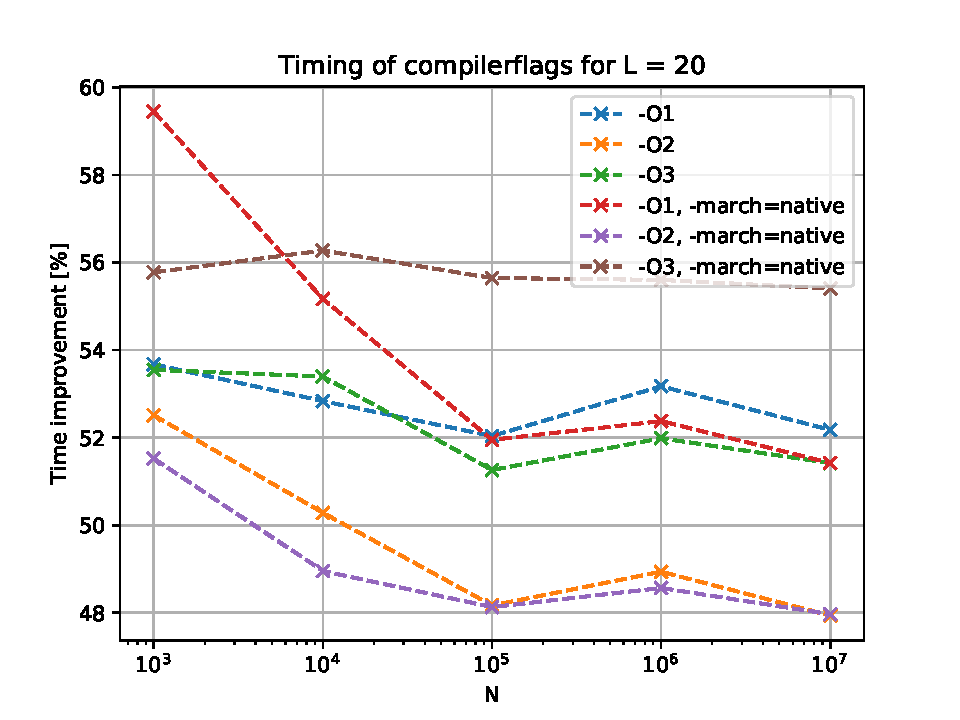
\includegraphics[width=\columnwidth]{../data/benchmark.pdf}
	\caption{Time improvement in percentage of various compiler optimization flags for a \(20\times 20\) lattice with \(8\) evenly spaced values of \(T \in [2.20, 2.35]\). All results are achieved with parallelized runs with \(8\) threads (one value of \(T\) per thread)} \label{fig:benchmark_compiler_flags}
\end{figure}



\subsection{Simulation with a $2\times 2$ lattice} \label{sec:IV:B}


\subsection{Simulations with a $20 \times 20$ lattice} \label{sec:IV:C}

In order to evaluate the stability and convergence of our solver we simulated a $20 \times 20$ lattice of spins with temperatures $T = 1$ and $T = 2.4$ (in units of $k_B T/J$). We ran these simulations with both an ordered intial state (all spins pointing up) and a disordererd initial state (randomized spin configuration). 


\begin{figure}[H]
\centering
\includegraphics[width=\columnwidth]{{"../data/ordered initial spin.-t1.0-20x20-E"}.pdf}
\includegraphics[width=\columnwidth]{{"../data/unordered initial spin.-t1.0-20x20-E"}.pdf}
\caption{This figure contains plots of averaged energy as a function of amount of Monte Carlo cycles performed for simulations with a $20\times 20$ lattice and temperature $T=1$ (in units of $k_B T/J$). The first plot shows the development of the energy when the initial state is ordered (all spins pointing up) and the second plot shows the energy when the initial state is disordered (randomized spin configuration).} \label{fig:20x20-T1.0-energy}
\end{figure} 

\begin{figure}[H]
\centering
\includegraphics[width=\columnwidth]{{"../data/ordered initial spin.-t1.0-20x20-|M|"}.pdf}
\includegraphics[width=\columnwidth]{{"../data/unordered initial spin.-t1.0-20x20-|M|"}.pdf}
\caption{This figure contains plots of the averaged absolute of the magnetization as a function of amount of Monte Carlo cycles performed for simulations with a $20\times 20$ lattice and temperature $T=1$ (in units of $k_B T/J$). The first plot shows the development of the magnetization when the initial state is ordered (all spins pointing up) and the second plot shows the magnetization when the initial state is disordered (randomized spin configuration).} \label{fig:20x20-T1.0-absolute_magnetization}
\end{figure} 

\begin{figure}[H]
\centering
\includegraphics[width=\columnwidth]{{"../data/ordered initial spin.-t1.0-20x20-Nconf"}.pdf}
\includegraphics[width=\columnwidth]{{"../data/unordered initial spin.-t1.0-20x20-Nconf"}.pdf}
\caption{This figure contains plots of the total amount of accepted configurations as a function of amount of Monte Carlo cycles performed for simulations with a $20\times 20$ lattice and temperature $T=1$ (in units of $k_B T/J$). The first plot shows the amount of accepted configurations when the initial state is ordered (all spins pointing up) and the second plot shows amount of accepted configurations when the initial state is disordered (randomized spin configuration).} \label{fig:20x20-T1.0-Nconf}
\end{figure}

\begin{figure}[H]
\centering
\includegraphics[width=\columnwidth]{{"../data/ordered initial spin.-t1.0-20x20-PE"}.pdf}
\includegraphics[width=\columnwidth]{{"../data/unordered initial spin.-t1.0-20x20-PE"}.pdf}
\caption{This figure contains plots of the numerically calculated probability distribution of the energy with a $20\times 20$ lattice and temperature $T=1$ (in units of $k_B T/J$). The first plot shows the probability distribution when the initial state is ordered (all spins pointing up) and the second plot shows the probability distribution when the initial state is disordered (randomized spin configuration).} \label{fig:20x20-T1.0-PE}
\end{figure} 


\begin{figure}[H]
\centering
\includegraphics[width=\columnwidth]{{"../data/ordered initial spin.-t2.4-20x20-E"}.pdf}
\includegraphics[width=\columnwidth]{{"../data/unordered initial spin.-t2.4-20x20-E"}.pdf}
\caption{This figure contains plots of averaged energy as a function of amount of Monte Carlo cycles performed for simulations with a $20\times 20$ lattice and temperature $T=2.4$ (in units of $k_B T/J$). The first plot shows the development of the energy when the initial state is ordered (all spins pointing up) and the second plot shows the energy when the initial state is disordered (randomized spin configuration).} \label{fig:20x20-T2.4-energy}
\end{figure} 

\begin{figure}[H]
\centering
\includegraphics[width=\columnwidth]{{"../data/ordered initial spin.-t2.4-20x20-|M|"}.pdf}
\includegraphics[width=\columnwidth]{{"../data/unordered initial spin.-t2.4-20x20-|M|"}.pdf}
\caption{This figure contains plots of the averaged absolute of the magnetization as a function of amount of Monte Carlo cycles performed for simulations with a $20\times 20$ lattice and temperature $T=2.4$ (in units of $k_B T/J$). The first plot shows the development of the magnetization when the initial state is ordered (all spins pointing up) and the second plot shows the magnetization when the initial state is disordered (randomized spin configuration).} \label{fig:20x20-T2.4-absolute_magnetization}
\end{figure} 

\begin{figure}[H]
\centering
\includegraphics[width=\columnwidth]{{"../data/ordered initial spin.-t2.4-20x20-Nconf"}.pdf}
\includegraphics[width=\columnwidth]{{"../data/unordered initial spin.-t2.4-20x20-Nconf"}.pdf}
\caption{This figure contains plots of the total amount of accepted configurations as a function of amount of Monte Carlo cycles performed for simulations with a $20\times 20$ lattice and temperature $T=2.4$ (in units of $k_B T/J$). The first plot shows the amount of accepted configurations when the initial state is ordered (all spins pointing up) and the second plot shows amount of accepted configurations when the initial state is disordered (randomized spin configuration).} \label{fig:20x20-T2.4-Nconf}
\end{figure}

\begin{figure}[H]
\centering
\includegraphics[width=\columnwidth]{{"../data/ordered initial spin.-t2.4-20x20-PE"}.pdf}
\includegraphics[width=\columnwidth]{{"../data/unordered initial spin.-t2.4-20x20-PE"}.pdf}
\caption{This figure contains plots of the numerically calculated probability distribution of the energy with a $20\times 20$ lattice and temperature $T=2.4$ (in units of $k_B T/J$). The first plot shows the probability distribution when the initial state is ordered (all spins pointing up) and the second plot shows the probability distribution when the initial state is disordered (randomized spin configuration).} \label{fig:20x20-T2.4-PE}
\end{figure} 



\subsection{Simulations with larger lattice sizes} \label{sec:IV:D}





\newpage

\section{Discussion} \label{sec:V}


\newpage

\section{Conclusion} \label{sec:VI}


\onecolumngrid
\bibliography{kilder.bib}{}
\newpage
\twocolumngrid

\appendix
\section{Source code} \label{A}
All code for this report was written in C++ and Python 3.8, and the complete set of files can be found at
\url{https://github.com/eivinsto/FYS3150_Project_4.git}.

\cprotect\subsection{\verb+ising_metropolis.hpp+} \label{A.1}

\cprotect\subsection{\verb+ising_metropolis.cpp+} \label{A.2}

\cprotect\subsection{\verb+main.cpp+} \label{A.3}

\cprotect\subsection{\verb+python.py+} \label{A.4}

\cprotect\subsection{\verb+test_functions.py+} \label{A.5}

\newpage
\section{Selected results} \label{B}
Here is a folder of selected results from running our code.

\url{https://github.com/eivinsto/FYS3150_Project_4/tree/master/data}

~
\newpage
\section{System specifications} \label{C}
All results included in this report were achieved by running the implementation on the following system:

\begin{itemize}
	\item CPU: AMD Ryzen \(9\) \(3900\)X
	\item RAM: \(2\times\SI{8}{\giga\byte}\) Corsair Vengeance LPX DDR\(4\) \(\SI{3200}{\mega\hertz}\)
\end{itemize}

\end{document}
